\svnid{$Id$}
\chapter{Model - Construction and Parameters}
\label{chap:model}
\section{Construction}

The model was constructed based on existing knowledge of the respiratory chain in \Nsm{} from the ETC shown in Figure \ref{fig:etc} (Chapter \ref{chap:intro}). No \textit{a priori} assumptions are made about separation of time-scales that would permit the use of Michaelis-Menten kinetics, as the rates of intermediate reaction steps are not known. This approach also permits tracking of the oxidation state of all the intermediates which allows understanding and offers the potential for predictions that may be explored in future \textit{in vivo} studies.

The model was generated as a set of ordinary differential equations which describe the bulk-average concentration of substrates, products, enzymes and their activity within a well-mixed vessel. It is assumed that the bacterial population structure is homogeneous and that there are no variations in concentrations of substrates between the bulk media and within the bacterial cells. Stochastic effects are ignored at the protein level, but they are unlikely to be of importance. Initially protein production is largely ignored as the switching mechanism is thought to happen on a time-scale that is much shorter than the transcription and translation of new proteins, they are therefore assumed to be expressed constitutively except where stated otherwise. However some datasets were available in the published literature\cite{Rock2005} that suggested otherwise, and were tested using an extension to the model described below which includes transcription and translation of certain components.

\subsection{Normalising the Data}
The model contains no implied information about cell density. This means the values for various component concentrations will differ between experiments.
Initially the optical density of cultures was used to determine the cell density however experiments proved that this was not a completely reliable proxy as the optical density is also affected by dead cells. Using optical density as a cell density proxy should give linear relationships between cell densities and overall reduction rates, however this proved not to be the case, with rates of oxygen reduction differing between cultures with the same optical density (data not shown). Therefore where possible, any normalisation that was carried out used the initial oxygen reduction rate as a relative indicator of living cells. Plating out serial dilutions of high density cultures showed that a culture with $OD_{600} = 1$ contains approximately $1 \times 10^9$ cells/ml.

%The model contains no implied information about cell density. This means the values for various component concentrations will differ between experiments. Initially the optical density of cultures was used to determine the cell density however experiments proved that this was not a completely reliable proxy for cell density as this also includes dead cells. Using optical density as a cell density proxy should haven given linear relations between cell densities and reaction rates, however this proved not to be the case, with rates of oxygen reduction different between cultures with the same optical density. Therefore where possible, any normalisation that was carried out used the initial oxygen reduction rate as a relative indicator.

\subsection{Converting Biological Reactions into Differential Equations}
The rationale for obtaining the form for each of the 9 component equations is described below. Throughout the model the reduced components, i.e. those with available electrons, are denoted as active and have a subscript $a$. Components lacking a subscript denote the total, constant, amount of a component. $\emptyset$ denotes nothing (this is used as the source or sink when substrates are entering or exiting the system).

\subsubsection{Respiratory Substrates}
{\bf Oxygen}\\
The change in concentration of oxygen is affected by the following kinetic processes.
\begin{equation*}
\begin{gathered}
\emptyset\xrightarrow{\beta} O_2\\
O_2 + C_a\xrightarrow{k_1} H_{2}O + C_i
\end{gathered}
\end{equation*}
where $\beta$ is the rate constant of passive diffusion (as a function of \cOxygen{} concentration) of \cOxygen{} into the electrode chamber. The rate constant $k_1$ describes the reduction of oxygen by the oxygen reductase \cbbthree{}; this value depends on the concentration of reduced (i.e. active) \cbbthree{}, $C_a$ and the concentration of $O_2$.
The differential equation that gives the change in oxygen concentration is
\begin{equation}
\frac{d[O_2]}{dt} = \beta(1-[O_2]/K_O) - k_{1}[C_a][O_2]
\label{eq:oxygen}
\end{equation}
In isolation the first term gives rise to a simple exponential input of oxygen until the saturation level ($K_O$) is reached to account for diffusion into the system. The rationale for the form of the equation is given below.\\
\noindent
During the course of the experimental stages of this work, on occasions where the respiring cultures had died, either through being left in essentially anaerobic conditions for too long, or were treated with Chloramphenicol (which stops all protein production in the cell), the oxygen levels in the culture media would begin to rise slowly. This did not occur in every case, and after some further experimentation it was concluded that it probably occurs when an air bubble gets trapped underneath the lid of the oxygen electrode chamber. To try and abate the rate of diffusion in all subsequent experiments particular care was taken to avoid an air bubble being trapped in the electrode chamber.

Unfortunately even with no air bubble a small amount of oxygen was diffusing in, so an experiment was set up to try and quantify the rate of diffusion. Wild-type \Nm{} cultures were grown to various different cell densities and left to respire aerobically. Once the cultures had used all the available oxygen they were killed either by adding a small volume of Potassium Cyanide ($50 \mu l$ of a $50 \mu M$ solution), or by heating the culture to 95 \textdegree{}C for 10 minutes. Oxygen concentrations were then recorded as the gas diffused back into the electrode chamber.% It should be noted that Chloramphenicol should not actually kill the cells as it merely prevents further protein production in the cell, however the results of this experiment showed that under anaerobic conditions after addition of Chloramphenicol the cultures are no longer capable of respiring oxygen.

The experimental data showed that the increasing oxygen concentration takes the form of an inverse exponential decay and therefore can be fit very easily to an exponential function. The exact parameters of the diffusion seem to differ between cultures but it appeared to have a dependence on the cell density whereby lower cell densities generally had higher rates of diffusion than higher cell densities, but there was no obvious direct relationship.
The equation used to fit raw data for oxygen diffusion is a 3 parameter exponential:
\begin{equation*}
f(x) = c - ae^{-bx}
\end{equation*}
In the differential equation this collapses to two parameters, the oxygen saturation level, and the rate of oxygen recovery thus:
\begin{equation*}
\dfrac{d[O_2]}{dt} = \beta(1-O_2/K_O)
\end{equation*}
Integrating and separating this equation gives:
\begin{equation*}
\begin{gathered}
-\beta\dfrac{t}{K_O} + C = ln([O_2]-K_O)\\
\Rightarrow [O_2]-K_O = Ae^{\left(-\beta\dfrac{t}{K_O}\right)}\\
\Rightarrow [O_2] = K_O + Ae^{\left(-\beta\dfrac{t}{K_O}\right)}
\end{gathered}
\end{equation*}
\clearpage
\noindent{\bf Nitric Oxide}\\
The change in nitric oxide concentration is affected by the following kinetic processes.
\begin{equation*}
\begin{gathered}
NO_2^- + A_a \xrightarrow{m_1} NO + A_i\\
NO + B_a \xrightarrow{l_1} N_2O + B_i\\
NO + C_a \xrightarrow{k_5} NO\mhyphen C_X\\
NO\mhyphen C_X \xrightarrow{k_6} NO + C_a\\
NO \xrightarrow{\gamma} \emptyset
\end{gathered}
\end{equation*}
The equations above have a number of additional interactions in comparison to $\mathrm{O}_2$. NO is created by the reduction of $\mathrm{NO}_\mathrm{2}^\mathrm{-}$ by AniA, is reduced by its dedicated reductase, NorB, and converted to $\mathrm{N}_2\mathrm{O}$ which is lost from the cell, interacts with \cbbthree{}, and is also spontaneously lost from the electrode chamber. It is assumed that the interaction with \cbbthree{} occurs only in a reversible manner, leading to an NO bound and temporarily inactive form $C_X$. There is evidence that this interaction can also lead to permanent degradation of \cbbthree{} via the formation of peroxynitrite at the terminal oxidase\cite{Sharpe1998,Blomberg2005}. This is not currently considered in this version of the model. These effects are described mathematically in the equation below.
%The equation for describing \cNO{} concentration changes is more complex as \cNO{} has a number of additional interactions in comparison to \cOxygen{}. \cNO{} also interacts with \cbbthree{}, in addition to being reduced from \cNitrite{}, reduced to \cNtwoO{} and spontaneously lost from the electrode chamber. Currently this is the equation being used to model \cNO{} concentration.
\begin{equation}
\frac{d[NO]}{dt} = m_{1}[NO_2^-][A_a] - l_1[NO][B_a] - k_5[C_a][NO] + k_6 [C_X] - \gamma[NO]
\label{eq:no}
\end{equation}
The rate of synthesis of NO is captured by the first term, with rate constant $m_{1}$ and depends on the both the concentration of $\mathrm{NO}_\mathrm{2}^\mathrm{-}$ and reduced AniA ($A_a$). The reduction of NO is described by the next term with the rate constant $l_1$ and also depends on the concentration of NO and reduced NorB ($B_a$). Inhibition of \cbbthree{} by NO is modelled by the $\mathrm{3}^\mathrm{rd}$ component of the equation. $k_5$ is the rate constant describing the reversible binding of NO to \cbbthree{} to form the inactive form of \cbbthree{}, $C_X$. $k_6$ is the rate of recovery of this inhibited \cbbthree{}. $\gamma$ is the spontaneous rate of loss of NO from the electrode chamber.\\
%The synthesis of \cNO{} is modelled by $m_{1}$ which is the rate of \cNitrite{} reduction by reduced (active) AniA. This also depends on the concentration of \cNitrite{} and reduced AniA ($A_a$). The reduction of \cNO{} requires $l_1$ which is the rate of reduction of \cNO{} by reduced (active) NorB. This depends on the concentration of \cNO{} and reduced NorB ($B_a$). Inhibition of \cbbthree{} by \cNO{} is modelled by the \engordnumber{3} component of the equation. $k_5$ is the rate of inhibition of \cbbthree{} by \cNO{}. $k_6$ is the rate of recovery of inhibited \cbbthree{}. $\gamma$ is the rate of spontaneous loss of \cNO{} from the electrode chamber.
\clearpage
\noindent{\bf Nitrite}\\
The change in nitrite concentration is affected by the following kinetic process.
\begin{equation*}
NO_2^- + A_a \xrightarrow{m_1} NO + A_i
\end{equation*}
Which can be modelled mathematically by this equation
\begin{equation}
\frac{d[NO_2^-]}{dt} = - m_{1}[NO_2^-][A_a]
\label{eq:nitrite}
\end{equation}
where $m_{1}$ is the rate constant for reduction of \cNitrite{} by reduced (active) AniA ($A_a$).

\subsubsection{Electron Transporters}

In addition to the rate of change of concentration of the respiratory substrates, the model also contains information about the upstream state of components of the transfer chain, starting from the quinone pool. The ultimate upstream source of electrons into the respiratory chain is from NADH, but for the sake of simplicity all processes prior to the quinone pool are subsumed into a simple single rate constant. This simplification is made to avoid further complications associated with varying metabolism and to avoid distraction from the stated primary aim of understanding the switching behaviour of the downstream chain. The quinone pool was chosen as the starting point because it is known that NorB draws electrons directly from this point and therefore this represents the first branch in the chain. The desire was to understand how competition for electrons at branches affects function and therefore the quinone pool is included in the model.\\
%In addition to the rate of change of concentration of the respiratory substrates, the model also contains information about the state of the quinone pool, which is the upstream source of electrons into the respiratory chain. This is important because this affects the rate of reduction of the various enzymes which perform the substrate reductions. The equation for modelling the change in reduction state (activity) of the quinone pool is
\clearpage
\noindent{\bf Quinones}\\
The change in concentration of reduced quinones is affected by the following kinetic processes.
\begin{equation*}
\begin{gathered}
Q_i \xrightarrow{g} Q_a\\
B_i + Q_a \xrightarrow{l_3} B_a + Q_i\\
X_i + Q_a \xrightarrow{f} X_a + Q_i
\end{gathered}
\end{equation*}
The differential equation that models these reactions is
\begin{equation}
\frac{d[Q_a]}{dt} = g([Q] - [Q_a]) - l_3[Q_a]([B] - [B_a]) - f[Q_a]([X]-[X_a])
\label{eq:quinones}
\end{equation}
$Q_a$ is the reduced quinone, and $Q$ the total concentration of quinones in the system ($Q_i$ is calculated from these two values). $g$ represents the constant rate of availability of electrons into the quinone pool from NADH. The reduction of NorB by active quinones is parametrised by the rate constant $l_3$. NorB and reduced NorB are given by $B$ and $B_a$ respectively. As the quinones also reduce the cytochromes, this also needs to be modelled. $f$ is the rate constant parametrising the reduction of cytochromes by the active quinones. Total cytochromes and total reduced cytochromes are given by $X$ and $X_a$ respectively which are used to calculated $X_i$ in the kinetic process.\\
{\bf Cytochromes}\\
A simplified version of cytochromes was used and therefore $X$ actually represents a pool of different cytochromes, \textit{c$_{\textrm{x}}$}, \textit{c$_{\textrm{4}}$}, \textit{c$_{\textrm{5}}$} and the \textit{bc$_{\textrm{1}}$} complex. These are amalgamated into one here to simplify the equations and focus on the simple branching of the chain and competition for electrons. This is a modelling choice and it is further discussed in Chapter \ref{chap:completedmodel}.
%$Q_a$ is the reduced quinone, and $Q$ the total concentration of quinones in the system. $g$ represents the rate of flow of electrons into the quinone pool from NADH. The rate of reduction of NorB by active quinones is given by $l_3$. NorB and reduced NorB are given by $B$ and $B_a$ respectively. As the quinones also reduce the cytochromes, this also needs to be modelled. $f$ denotes the rate of reduction of cytochromes by the active quinones. Cytochromes and reduced cytochromes are given by $X$ and $E$ respectively.

%Given that the concentration of active cytochromes changes, due to reduction by the quinone pool and oxidation by the downstream enzymes, and this concentration is a parameter in (\ref{eq:quinones}), it also needs to be included in the model, and this is given by the following equation
The concentration of active cytochrome pool changes due to both reduction by the upstream quinone pool and oxidation by both of the remaining downstream terminal enzymes can be seen in the following kinetic processes.
\begin{equation*}
\begin{gathered}
C_i + X_a \xrightarrow{k_3} C_a + X_i\\
A_i + X_a \xrightarrow{m_3} A_a + X_i\\
X_i + Q_a \xrightarrow{f} X_a + Q_i
\end{gathered}
\end{equation*}
These are modelled with the following differential equation
\begin{equation}
\frac{d[X_a]}{dt} = -k_3([C] - [C_a] - [C_X])[X_a]  - m_3([A] - [A_a])[X_a] + f[Q_a]([X]-[X_a])
\label{eq:cytochromes}
\end{equation}
where $k_3$ is the rate constant describing the reduction of the available oxidised cytochrome c oxygen reductase (\cbbthree{}) by the quinone pool (via \textit{c$_{\textrm{x}}$} \& \textit{c$_{\textrm{4}}$}). $C$, $C_a$ and $C_X$ represent the overall concentration of \cbbthree{}, reduced (active) \cbbthree{} and NO inhibited \cbbthree{} respectively. $m_3$ is the rate constant describing the reduction of AniA by the cytochrome pool (via \textit{c$_{\textrm{5}}$}). The concentration of active cytochromes is thus increased by their reduction by the quinone pool, but this in turn can reduce the flux from the pool because less oxidised cytochrome is available to accept electrons. As stated previously, the relative time scales are unknown so all processes appear explicitly.
%where $k_3$ is the rate of reduction of the cytochrome c oxygen reductase (\cbbthree{}) by the quinone pool (via \textit{c$_{\textrm{x}}$} \& \textit{c$_{\textrm{4}}$}). $C$, $C_a$ and $C_X$ represent the overall concentration of \cbbthree{}, reduced (active) \cbbthree{} and NO inhibited \cbbthree{} respectively. $m_3$ is the rate of reduction of AniA by the cytochrome pool (via \textit{c$_{\textrm{5}}$}). The concentration of active cytochromes increases by their reduction by the quinone pool.

\subsubsection{Terminal Reductases}
Finally the changes in concentration of reduced terminal oxidases, \cbbthree{}, AniA and NorB are described by the following equations. All the terms present in this section have been introduced previously. These equations of course could equally have been written for the oxidised form but these can easily be recovered because it is assumed that the total concentration of the oxidases remains constant.\\
%To model the changes in concentration of the individual enzymes, \cbbthree{}, AniA and NorB, the following equations are used:
\clearpage
\noindent{\bf Reduced \cbbthree{}}\\
The kinetic processes which affect the concentration of reduced (active) \cbbthree{} are
\begin{equation*}
\begin{gathered}
C_i + X_a \xrightarrow{k_3} C_a + X_i\\
O_2 + C_a\xrightarrow{k_1} H_{2}O + C_i\\
NO + C_a \xrightarrow{k_5} NO\mhyphen C_X\\
NO\mhyphen C_X \xrightarrow{k_5} NO + C_a
\end{gathered}
\end{equation*}
which is described by
\begin{equation}
\frac{d[C_a]}{dt} = k_3([C] - [C_a] - [C_X])[X_a] - k_{1}[C_a][O_2] - k_5[C_a][NO] + k_6[C_X]
\label{eq:active_cbb3}
\end{equation}
{\bf Inhibited \cbbthree{}}\\
The following kinetic process alters the concentrations of reversibly inhibited \cbbthree{}.
\begin{equation*}
\begin{gathered}
 NO + C_a \xrightarrow{k_5} NO\mhyphen C_X \xrightarrow{k_6} NO + C_a
\end{gathered}
\end{equation*}
which is described by
\begin{equation}
\frac{d[C_X]}{dt} = k_5[C_a][NO] - k_6 [C_X]
\label{eq:NO inhibited_cbb3}
\end{equation}
{\bf Reduced AniA}\\
The concentration of reduced AniA is affected by the following kinetic processes.
\begin{equation*}
\begin{gathered}
A_i + X_a \xrightarrow{m_3} A_a + X_i \\
NO_2^- + A_a \xrightarrow{m_1} NO + A_i
\end{gathered}
\end{equation*}
which can be modelled by
\begin{equation}
\frac{d[A_a]}{dt} = m_3([A] - [A_a])[X_a]- m_{1}[NO_2^-][A_a]
\label{eq:active_ania}
\end{equation}
{\bf Reduced NorB}\\
Changes in NorB concentration occur via the following kinetic processes.
\begin{equation*}
\begin{gathered}
B_i + Q_a \xrightarrow{l_3} Q_i + B_a \\
NO + B_a \xrightarrow{l_1} N_{2}O + B_i
\end{gathered}
\end{equation*}
and are modelled by this equation
\begin{equation}
\frac{d[B_a]}{dt} = l_3[Q_a]([B] - [B_a]) - l_1[NO][B_a]\\
\label{eq:active_norb}
\end{equation}


\subsection{Assumptions and their Justifications}
A number of assumptions were made regarding the kinetics and reactions taking place in the model.
\begin{enumerate}
 \item {\bf It is assumed that NO inhibits the reduced \cbbthree{} and not the oxidised form, since it is not expected that Nitric oxide to bind to an inactive enzyme.} This is corroborated by \citet{Giuffre2000}, who show significant levels of inhibition of reduced cytochrome. They do also however observe low levels of inhibition of the oxidised enzyme also. Their experiments used cytochrome c oxidase (aa3) rather than \cbbthree{}, but this assumption should still stand as the enzymes are of the same family. This also implies that the model deals exclusively with reversible inhibition.
 \item {\bf Bacterial population structure and concentration variation not considered.} The primary substrates of interest are gases and substrates which are thought to freely diffuse in and out of the cells. Additionally the culture is kept well-mixed at all times, thus it can be assumed that the culture is homogeneous.
 \item {\bf No backwards reactions.} For simplicity, backwards reactions are not included. However they may be important, and could easily be included in a future study with the concomitant increase in parameter count.
 \item {\bf No Michaelis-Menten kinetics.} Separation of time-scales cannot be assumed as the rates of intermediate reaction steps are not known. Future information regarding time-scale separation could easily be incorporated.
 \item {\bf All cytochromes can be modelled as one.} The main effort of modelling was to concentrate on the position of branches in the respiratory chain. In the same way the effects of Laz and $c_5$ on AniA and \cbbthree{} respectively are ignored. They are not the prime electron donors to their terminal reductases and contribute very little overall to the reduction\cite{Deeudom2007}. All the electron donors are treated as a single modelled entity.
\end{enumerate}

%Also, values are in the right ball park even though they are using aa3 rather than \cbbthree. $10^8 M ^{-1} s ^{-1}$ against around $50 \mu M ^{-1} s ^{-1}$.

\section{Parameters and their Prior Distributions}

None of the rate constants or concentrations which were required for this model have previously been determined for \Nsm, so values from other similar organisms had to be used instead. In some cases there appears to be no data in the literature regarding values of particular components. Table \ref{tab:ps} lists the values that have been obtained from the literature.

\begin{table}[tbp]
\begin{center}
\begin{tabular}{>{\centering}m{1.6cm}>{\centering}m{6.1cm}>{\centering}m{2.5cm}>{\centering}m{3.1cm}}
\toprule
\textbf{Symbol} & \textbf{Description} & \textbf{Value} & \textbf{Source}
\tabularnewline
\midrule
$k_1$ & Rate constant for O$_{\textrm{2}}$ reduction by reduced \cbbthree{} & $415~\mu M^{-1} s^{-1}$ & \citet{Forte2001} and \citet{Hunter2007}
\tabularnewline\noalign{\smallskip}\hline\noalign{\smallskip}

$k_3$ & Rate constant for \cbbthree{} reduction by cytochrome pool & $3~\mu M^{-1} s^{-1}$ & \citet{Chang2010}
\tabularnewline\noalign{\smallskip}\hline\noalign{\smallskip}

$l_1$ & Rate constant for NO reduction by reduced NorB & $0.9 - 500~\mu M^{-1} s^{-1}$ & \citet{Rock2007} and \citet{Wasser2002}
\tabularnewline\noalign{\smallskip}\hline\noalign{\smallskip}

$l_3$ & Rate constant for NorB reduction by quinone pool & Unknown & N/A
\tabularnewline\noalign{\smallskip}\hline\noalign{\smallskip}

$m_1$ & Rate constant for NO$_{\textrm{2}}^{\textrm{-}}$ reduction by reduced AniA & Unknown & N/A
\tabularnewline\noalign{\smallskip}\hline\noalign{\smallskip}

$m_3$ & Rate constant for AniA reduction by cytochrome pool & $4.8\pm0.2~\mu M^{-1}s^{-1}$ & \citet{Nojiri2009}
\tabularnewline\noalign{\smallskip}\hline\noalign{\smallskip}

$k_5$ & Rate constant for \cbbthree{} inhibition by NO & $100~\mu M ^{-1} s ^{-1}$ & \citet{Giuffre2000} and \citet{Blackmore1991}
\tabularnewline\noalign{\smallskip}\hline\noalign{\smallskip}

$k_6$ & Rate constant for recovery of NO inhibited \cbbthree{} & $38~s^{-1}$ & \citet{Rock2005}
\tabularnewline\noalign{\smallskip}\hline\noalign{\smallskip}

$\beta$ & Rate constant for passive diffusion in of O$_{\textrm{2}}$ & Unknown & N/A
\tabularnewline\noalign{\smallskip}\hline\noalign{\smallskip}

$K_O$ & Saturation O$_{\textrm{2}}$ level & $48~\mu M$ & This work
\tabularnewline\noalign{\smallskip}\hline\noalign{\smallskip}

$g$ & Rate of electrons in from NADH & $0.8~s^{-1}$ & This work
\tabularnewline\noalign{\smallskip}\hline\noalign{\smallskip}

$f$ & Rate constant for reduction of cytochromes by quinones & $8~\mu M^{-1}s^{-1}$ & This work
\tabularnewline\noalign{\smallskip}\hline\noalign{\smallskip}

$\gamma$ & Spontaneous loss of NO & Unknown & N/A
\tabularnewline\noalign{\smallskip}\hline\noalign{\smallskip}

$Q$ & Concentration of quinones & $0.3~\mu M$ & \citet{Hedrick1986}
\tabularnewline\noalign{\smallskip}\hline\noalign{\smallskip}

$X$ & Concentration of cytochromes & $\approx3.97~\mu M$ & \citet{Deeudom2007}
\tabularnewline\noalign{\smallskip}\hline\noalign{\smallskip}

$A$ & Concentration of AniA & $0.003 - 0.03~\mu M$ & This work
\tabularnewline\noalign{\smallskip}\hline\noalign{\smallskip}

$B$ & Concentration of NorB & $0.003 - 0.03~\mu M$ & This work
\tabularnewline\noalign{\smallskip}\hline\noalign{\smallskip}

$C$ & Concentration of \cbbthree{} & $0.003 - 0.03~\mu M$ & This work
\tabularnewline
\bottomrule
\end{tabular}
\caption[Model parameters]{{\bf Model parameters.} This table shows all the parameter values that have been obtained from the extant literature, or interpolated from preliminary experiments done during the course of this work. These values represent the initial data that is used to populate the model, from which all subsequent parameter sets are generated. For values that show concentrations of components, they represent the value for a culture with $OD_{600}=1.00$.
\label{tab:ps}}
\end{center}
\end{table}

\subsection*{Variables}
\subsubsection*{$\mathbf{O_2}$ {\bf- Oxygen concentration}}
This variable is always obtained directly from the experimental dataset as it indicates the starting point for oxygen in the model. It is calculated from a linear regression analysis of the first linear section of oxygen reduction to eliminate noise in the data.

\subsubsection*{$\mathbf{NO}$ {\bf- Nitric oxide concentration}, and $\mathbf{NO_2^-}$ {\bf- Nitrite concentration}}
As for Oxygen concentration, these variables are simply obtained from the dataset and the same conditions apply.

\subsubsection*{$\mathbf{X_a}$, $\mathbf{A_a}$, $\mathbf{B_a}$, $\mathbf{C_a}$, $\mathbf{Q_a}$ - Reduced enzyme concentrations, and $\mathbf{C_X}$ {\bf- Reversibly NO inhibited \cbbthree{}}}
These values are unknown at start of simulations. They have to be lower than the total concentrations for each enzyme, and the model enforces this. Given the rates of reduction of these enzymes they are all set to very low values, determined from exploratory runs of the parameter estimation algorithm. The rates of reduction for these enzymes actually make the initial value (so long as it is low) largely irrelevant as they reach their steady-state after only a few integration cycles.

\subsection*{Parameters}
\subsubsection*{$\mathbf{k_1}$ {\bf- Rate constant for O$_{\textrm{2}}$ reduction by reduced \cbbthree{}}}
%\citet{Preisig1996} show that \textit{B. japonicum} \cbbthree{} (\textit{fixNOQP}) has a $K_m$ of $55.7 \pm 24.2$ nM $\mathrm{O}_2$, and $V_{max}$ $37.4 \pm 9.2$ $\mathrm{nmol O}_2 \mathrm{min}^{-1} \mathrm{mg}^{-1}$.\\
%Given $v = \frac{V_{max}[S]}{K_m+[S]}$
%Then at high $O_2$ rate is:
%$v = \frac{37.4\times 100,000}{55.7+100,000} = 37.4~nmol^{-1}min{-1}mg{-1} = 0.000622986~\mu mol^{-1}s{-1}mg{-1}$\\

A value for $k_1$, the constant for O$_{\textrm{2}}$ reduction by reduced \cbbthree{} was calculated by using the $\mathrm{K}_{cat}$ value from \textit{Pseudomonas stutzeri}, and the $\textrm{k}_m$ value from \textit{Neisseria lactamica}, which \citet{Forte2001} and \citet{Hunter2007} determine are $166~s^{-1}$ and $0.4~\mu M$ respectively. $k_1$ can be calculated as $\frac{166~s^{-1}}{0.4~\mu M} = 415~\mu M^{-1}s^{-1}$.

\subsubsection*{$\mathbf{k_3}$ {\bf- Rate constant for \cbbthree{} reduction by cytochrome pool}}
$k_3$, the rate constant for reduction of \cbbthree{} by the cytochromes was calculated from values obtained from the maximum reduction rate of \cbbthree{} by cytochrome $c_4$ in \textit{Vibrio cholerae} by \citet{Chang2010}. A rate of 300 electrons transported per second was observed with a cytochrome $c_4$ concentration of $100~\mu M$. This concentration was not saturating, but there appears to be a linear relationship between rate and concentration. It is assumed that 1 electron equals 1 reduction of \cbbthree{}, thus the rate constant for reduction of \cbbthree{} by cytochromes is $\frac{300~s^{-1}}{100~\mu M} = 3~\mu M^{-1}s^{-1}$.

\subsubsection*{$\mathbf{l_1}$ {\bf- Rate constant for NO reduction by reduced NorB}}
%240 and 256 nanomoles NO reduced per minute per OD600 unit as determined by \citet{Barth2009}.

An estimate for the rate constant for NO reduction by reduced NorB can be obtained from \citet{Rock2007}.\\
\noindent They observed rates of NO reduction of $54 \pm 6~\mathrm{nmolmin}^{-1} \mathrm{mg}^{-1}$  in total protein content from dry weight. Thus the rate of NO reduction is $0.9 \pm 0.1~\mu\mathrm{mol~s}^{-1}\mathrm{g}^{-1}$ bacterial protein. The protein content of the cells was assumed to be similar to that of \textit{E. coli} at 50\% of dry weight, where each cell weighed 2 pg. A culture of \textit{Neisseria meningitidis} with $OD_{600} = 1$ has $1 \times 10^9~\textrm{cells/ml}$, and the reaction volume is 5 ml. $5\times 10^9~\textrm{cells} \times 2\times 10^{-12}~\textrm{g} \times 50\% \times 0.9~\mu\mathrm{mol~ s}^{-1}\mathrm{g}^{-1}$ results in $4.5~nmol~s^{-1}$ of quinones in 5ml, which when converted to molarity is $0.9~\mu M^{-1} s^{-1}$.

\citet{Wasser2002} suggest that the rate constant may be as high as $500~\mu M^{-1} s^{-1}$, although this was estimated for a cNOR type nitric oxide reductase.

\subsubsection*{$\mathbf{l_3}$ {\bf- Rate constant for NorB reduction by quinone pool}}
No information available in the literature, so the rate constant is set to $1~\mu M^{-1}s^{-1}$.

\subsubsection*{$\mathbf{m_1}$ {\bf- Rate constant for NO$_{\textrm{2}}^{\textrm{-}}$ reduction by reduced AniA}}
No information available in the literature, so the rate constant is set to $1~\mu M^{-1}s^{-1}$.

\subsubsection*{$\mathbf{m_3}$ {\bf- Rate constant for AniA reduction by cytochrome pool}}
The value for $m_3$, the rate constant for reduction of AniA by cytochromes, is the observed electron transfer rate between the equivalent cytochrome and nitrite reductase from \textit{Achromobacter xylosoxidans}. A value of $4.8\pm0.2~\mu M^{-1}s^{-1}$ was observed during stopped-flow experiments by \citet{Nojiri2009}.

\subsubsection*{$\mathbf{k_5}$ {\bf- Rate constant for \cbbthree{} inhibition by NO}}
\citet{Giuffre2000} and \citet{Blackmore1991} showed with cytochrome \textit{c} oxidase that NO could bind reversibly and inhibit the activity of the enzyme. The rate constant they calculated was $10^8~M ^{-1} s ^{-1}$. An assumption was made that even though the enzyme is different, its NO binding characteristics would be similar to that of \cbbthree{} as it is of the same family.

\subsubsection*{$\mathbf{k_6}$ {\bf- Rate constant for recovery of NO inhibited \cbbthree{}}}
\citet{Giuffre2000} calculated a half-life of t\textonehalf $\approx 80~\mathrm{min}$, however without any concrete values for concentration of $C_X\mhyphen NO$ this cannot be used to calculated a rate constant.
\citet{Rock2005} observed the apparent $K_i$ and calculated it to be 380 nM at $50~\mu M$ \cOxygen{}. Since $K_i = \frac{k_6}{k_5}$, a value for $k_6$ can be estimated as $k_6 = K_i \times k_5 = 0.38~\mu M \times 100~\mu M^{-1}s^{-1} = 38~s^{-1}$.

\subsubsection*{$\beta$ {\bf- Rate constant for passive diffusion in of O$_{\textrm{2}}$}, and $\mathbf{K_O}$ {\bf- Saturation O$_{\textrm{2}}$ level}}
The parameters obtained from fitting oxygen diffusion data showed a small difference in $K_O$ between cell densities, thus $K_O = 48~\mu M$ was selected as the standard value for this parameter. $\beta$ differed more between the experiments thus in the parameter estimation system is is not fixed and allowed to be modified freely. An example of the experimentally observed diffusion rates are shown in Figure \ref{fig:o2rec}.
\begin{figure}[tbp]
 \centering
 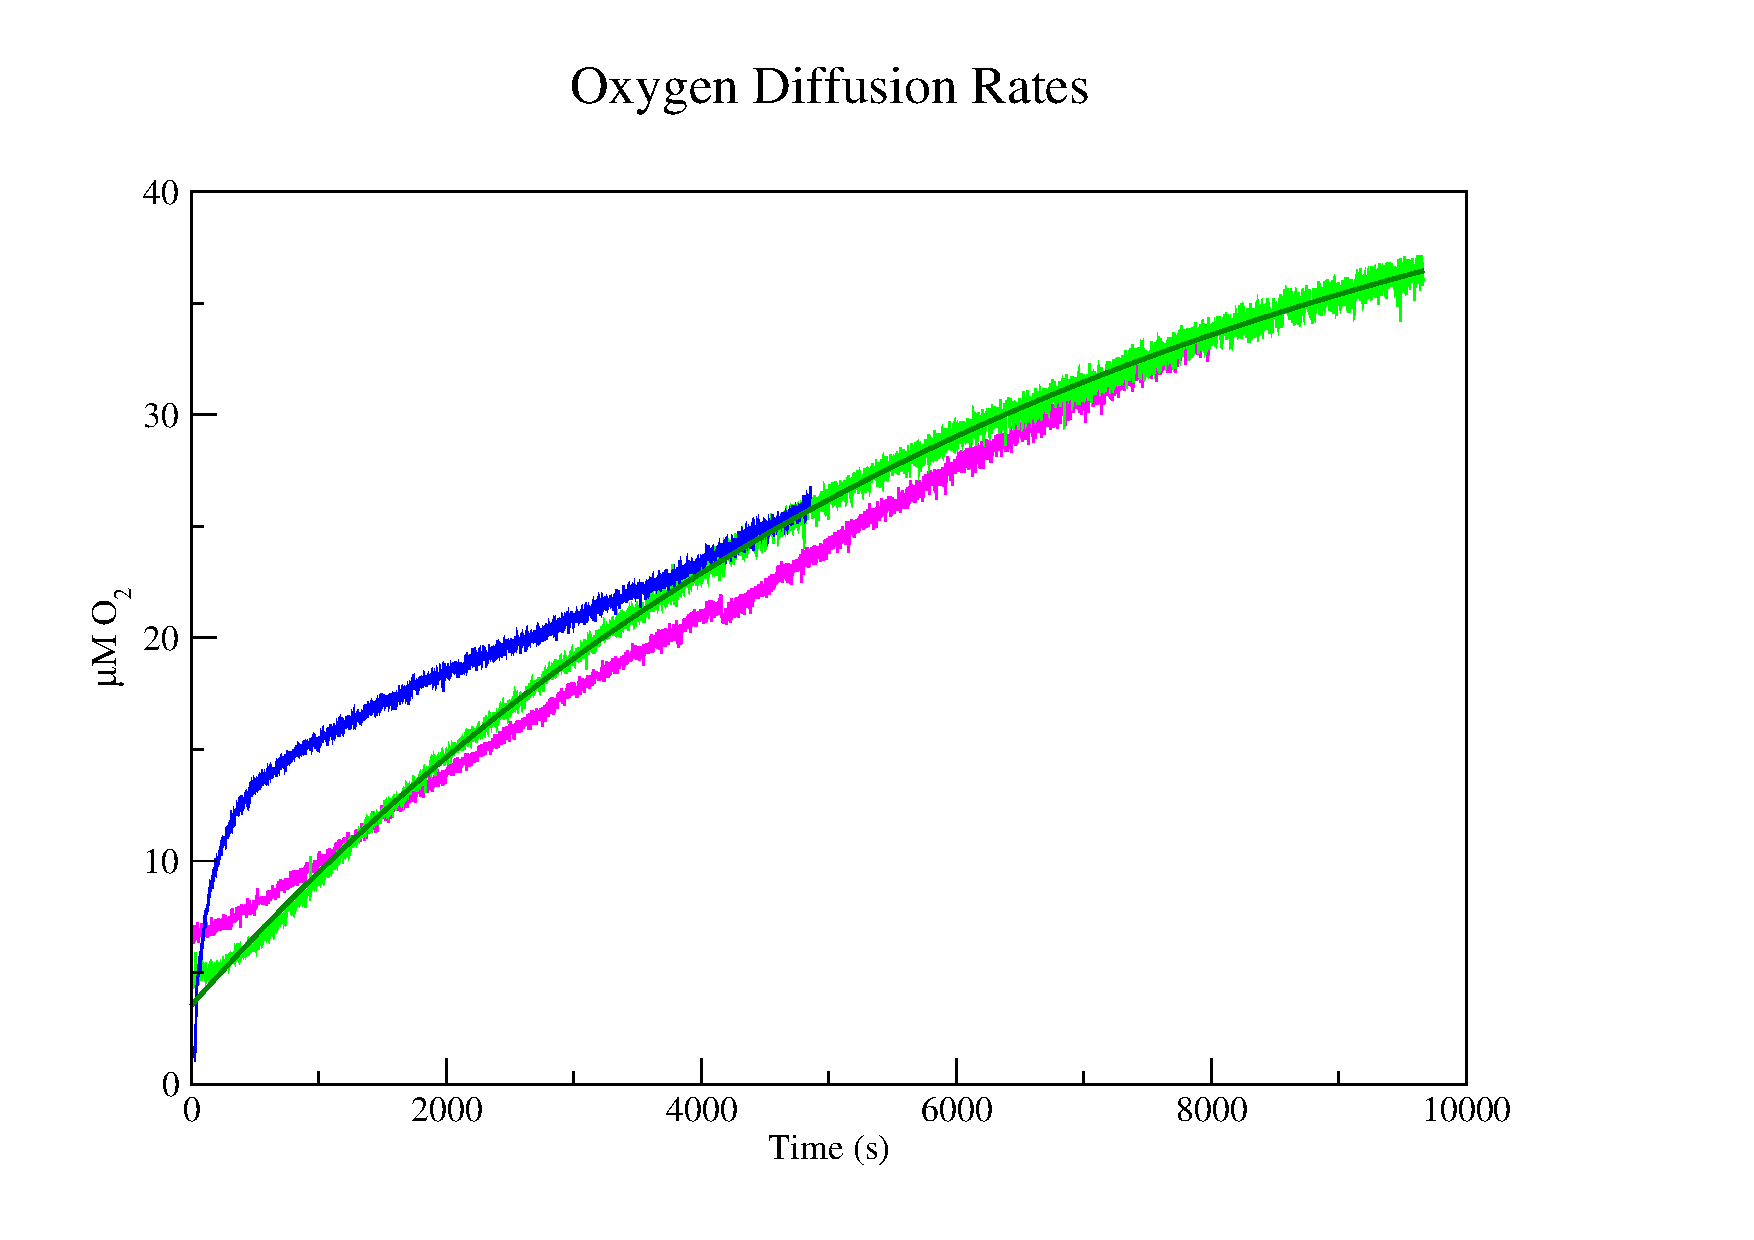
\includegraphics[width=14cm, trim=2cm 1cm 4cm 1cm]{./04-model/data/o2rec.pdf}
 % o2rec.pdf: 842x595 pixel, 72dpi, 29.70x20.99 cm, bb=0 0 842 595
 \caption[Oxygen Diffusion Rates]{{\bf Oxygen Diffusion Rates.} This figure shows experimentally observed rates of oxygen diffusion back into the electrode chamber. An exponential decay function has been fitted to the green dataset and produces the $K_O$ value of $\approx 48~\mu M$.
 \label{fig:o2rec}}
\end{figure}


\subsubsection*{$\mathbf{g}$ {\bf- Rate of electrons in from NADH (or rate of reduction of quinones)}}
This value is unknown, but initial runs of the algorithm suggest the value to be about $0.8~s^{-1}$.

\subsubsection*{$\mathbf{f}$ {\bf- Rate constant for reduction of cytochromes by quinones}}
\citet{Snyder2000} showed by reducing yeast cytochrome $\mathrm{bc}_1$ by using $25~\mu\mathrm{M}$ menaquinol the rate constants were $7.9~\mathrm{s}^{-1}$ for cytochrome b, and $1.55-6.9\times10^5~\mathrm{M}^{-1}\mathrm{s}^{-1}$ for cytochrome $\mathrm{c}_1$ (second order). However preliminary tests showed that a value of $8~\mu M^{-1}s^{-1}$ was more appropriate.

\subsubsection*{$\gamma$ {\bf- Spontaneous loss of NO}}
This value is assumed to be the same as the $\beta$, the rate constant for oxygen diffusion in across the liquid-gas barrier, as this is simply the reverse, given the physical similarity of Nitric Oxide and Oxygen.

\subsubsection*{$\mathbf{Q}$ {\bf- Concentration of quinones}}
$Q$, the concentration of quinones was calculated based on data from \citet{Hedrick1986}. The protein content of the cells was assumed to be similar to that of \textit{E. coli} at 15\% of wet weight, where each cell weighed 2 pg, and that there were $1\mu \textrm{mol}$ of respiratory quinones per g of bacterial protein\cite{Hollaender1977}. A culture of \textit{Neisseria meningitidis} with $OD_{600} = 1$ has $1 \times 10^9~\textrm{cells/ml}$, therefore there are 1.5 nmol of quinones in 5 ml culture ($5\times 10^9~\textrm{cells} \times 2\times 10^{-12}~\textrm{g} \times 15\% \times 1~\mu\textrm{mol/g}$), converted to molarity is $0.3~\mu M$.

\subsubsection*{$\mathbf{X}$ {\bf- Concentration of cytochromes}}
\citet{Deeudom2007} suggests that the total cytochrome concentration (inc. \cbbthree{}) is about $4~\mu M$ in \Nsm{}. Thus subtracting the value for C leaves a concentration of $\approx 3.97~\mu M$.

\subsubsection*{$\mathbf{A}$, $\mathbf{B}$, $\mathbf{C}$ {\bf- Concentration of Respiratory enzymes}}
Given the lack of concrete values for these parameters, the assumption is that all the respiratory enzymes are present in roughly equal quantities. Based on the values given for Q above, there are $1.5~mg$ of cell protein in 5 ml of $OD_{600}=1$ culture. \cbbthree{} is thought to be about 0.1-1\% of the total cell protein
%10\% of cell is membrane.
and is approximately 100 kDa in molecular weight. Therefore converting these values to molarity gives a concentration of approximately 3-30 nM.

\section{Solving Ordinary Differential Equations}
The model equations (given previously) are solved in parallel using the common $\mathrm{6}^\mathrm{th}$ order Runge-Kutta-Fehlberg algorithm for integrating ordinary differential equations\cite{Butcher2003}. Adaptive step-sizes were implemented using the Cash-Karp method\cite{Cash1990}. The adaptive step size system was required as it prevented the introduction of systemic numerical instabilities (see appendix for further details of why this was necessary).

%By keeping the quantities involved in their original state and not making any assumption about time-scale separation I am able to make predictions regarding the transient oxidation states of the various components. These are potentially experimentally accessible and appear to be crucial for the dynamic response of the chain in different environments.

\section{Implementation of the Model in Software}
The parameter estimation system and ODE solver were a bespoke implementation written in Java. The Runge-Kutta algorithm was modified from that found in Numerical Recipes in C\cite{Press1992}. A custom implementation was written rather than using off the shelf systems for solving ODEs and parameter estimation as maximum flexibility was required for integrating the two techniques (parameter estimation and ODE solving), and it allowed adaptation of the code to the requirements more quickly and more easily. Alternative systems are available such as COPASI \cite{Hoops2006}, but with more limited scope for customisation and integration of techniques.

The implementation of the model has no constraints on respiratory substrate concentration, thus allows the altering of these concentrations whilst solving the equations. % however changes to substrate concentration have to be made programmatically to inform the model of the change (\texttt{if (t == 50) then NO\_conc += 20;}).
This ability means that the switch between aerobic and anaerobic respiration can be examined synthetically, and the model is also capable of simulating how the respiratory system responds to the sudden addition of substrates such as Nitric Oxide. More complicated methods are possible, but given the high diffusion of the substrates concerned as well as the deliberate injection of the relevant substrate this method was a simpler and reasonable mimic for my empirical method. This ability was an absolute requirement, as in order to fully parametrise the model it was necessary to isolate sections of the model, which required adding aliquots of respiratory substrate during respiration.

%This ability means that the switch between aerobic and anaerobic respiration can be examined synthetically, and the model is also capable of simulating how the respiratory system responds to addition of substrates such as Nitric Oxide. This ability was an absolute requirement, as in order to fully parametrise the model it was necessary to isolate sections of the model, which required adding aliquots of respiratory substrate during respiration.

\section{Parameter Estimation}
Estimating the parameter values for the components in the mathematical model involved comparing the biological results with those produced by solving the ODEs and adjusting the parameter values to minimise the difference between the two results. The different methods for parameter estimation that were investigated are detailed in Chapter \ref{chap:paramest} [\nameref{chap:paramest}].